\documentclass[11pt]{article}
\usepackage[spanish]{babel}
\usepackage{amsmath, amssymb, bm}
\usepackage[a4paper,margin=2.5cm]{geometry}
\usepackage{graphicx}
\usepackage{hyperref}
\usepackage{float}


\newcommand{\ii}{\mathrm{i}}

\title{Tarea 4 Tecnologías Cuánticas}
\author{Juan Artigas,
    Antonia Dias,
    Lukas Wolff,
    Patricio Palacios,
    Manuel Tagle,
    Benjamin Tapia}
\date{}

\begin{document}
\maketitle

% =========================
\section{Scripts de Bob y Alice}

Se han desarrollado dos scripts, \texttt{alice\_choices.py} y \texttt{bob\_choices.py}, que generan las elecciones de bases para Alice y Bob, respectivamente. Estos scripts seleccionan específicamente los ángulos necesarios para el test CHSH: $0^\circ$ y $45^\circ$ para Alice, y $22.5^\circ$ y $-22.5^\circ$ para Bob. Para asegurar la reproducibilidad de los resultados, se utilizan semillas distintas: 1001 para Alice y 2002 para Bob.

Los archivos funcionan de la siguiente manera:

\section{Script del Árbitro}

El árbitro ejecuta el script \texttt{referee\_quantum.py}, que implementa el test de Bell usando el criterio CHSH (Clauser-Horne-Shimony-Holt). El proceso se desarrolla de la siguiente manera:

\subsection{Generación de Resultados Cuánticos}

Para cada par de mediciones con ángulos $\theta_A$ (Alice) y $\theta_B$ (Bob), el script simula un estado entrelazado Bell $|\Phi^+\rangle = \frac{1}{\sqrt{2}}(|00\rangle + |11\rangle)$ mediante la función \texttt{sample\_joint()}, que:

\begin{enumerate}
    \item Calcula la correlación teórica: $E = \cos(2(\theta_A - \theta_B))$
    \item Define las probabilidades cuánticas para los cuatro resultados posibles:
    \begin{align}
        P(+1,+1) &= P(-1,-1) = \frac{1+E}{4} \\
        P(+1,-1) &= P(-1,+1) = \frac{1-E}{4}
    \end{align}
    \item Muestrea aleatoriamente un resultado según estas probabilidades
\end{enumerate}

\subsection{Cálculo de Correlaciones}

El script calcula cuatro correlaciones específicas $E(a,b)$ para las combinaciones de bases del test CHSH:

\begin{itemize}
    \item $E(a,b)$: bases $a = 0^\circ$ y $b = 22.5^\circ$
    \item $E(a,b')$: bases $a = 0^\circ$ y $b' = -22.5^\circ$
    \item $E(a',b)$: bases $a' = 45^\circ$ y $b = 22.5^\circ$
    \item $E(a',b')$: bases $a' = 45^\circ$ y $b' = -22.5^\circ$
\end{itemize}

Para cada combinación de bases, la correlación se calcula como:
$$E(a,b) = \langle A_k \cdot B_k \rangle = \frac{1}{N} \sum_{k=1}^{N} A_k \cdot B_k$$

donde $A_k$ y $B_k$ son los resultados ($\pm 1$) de Alice y Bob para el par $k$, y $N$ es el número de mediciones para esa combinación específica de bases.

\subsection{Parámetro CHSH}

El parámetro CHSH se calcula como:
$$S = E(a,b) + E(a,b') + E(a',b) - E(a',b')$$

\textbf{Interpretación del parámetro CHSH:}
\begin{itemize}
    \item $|S| \leq 2$: Compatible con teorías de variables ocultas locales (límite clásico)
    \item $2 < |S| \leq 2\sqrt{2} \approx 2.828$: Violación de desigualdades de Bell, evidencia de entrelazamiento cuántico
    \item $|S| > 2\sqrt{2}$: Imposible según la mecánica cuántica (límite de Tsirelson)
\end{itemize}

\section{Resutados}

\subsection{Bases Iniciales}

Sobre las bases iniciales de Alice y Bob, se obtiene una correlacion de 2.77 lo que indica que se cumple el limite inferior de 2 y el superior de 2.828, lo que indica que tales bases se encuentran entrelazadas.

A continuacion se realizara el analisis sobre un conjunto de bases, donde se estudiara como se ven afectadas las correlaciones y el parametro CHSH.






\section{Descripción detallada del programa}

Implementamos la simulación de correlaciones cuánticas asociadas al estado de Bell $\ket{\Phi^+}$ mediante tres módulos fundamentales: generación de bases locales (Alice y Bob) y cálculo de correlaciones por parte de un árbitro. El código se desarrolló en Python utilizando \texttt{numpy} y \texttt{pandas} para el manejo de datos, y \texttt{matplotlib} para la visualización.

\subsection{Generación de bases locales}

\paragraph{Alice (función \texttt{generar\_bases\_alice\_df})}
Este módulo corresponde al \textbf{Script A}. Se reciben como entrada el número de pares $N$, las bases de Alice (por defecto $a=0^\circ$ y $a'=45^\circ$) y una semilla para el generador aleatorio (\texttt{seed=1001}).  
El programa genera un archivo \texttt{Alice\_choices.csv} con las columnas:
\[
\texttt{pair\_id}, \quad \texttt{Alice\_basis}
\]
donde cada fila corresponde a la elección aleatoria de una de las dos bases con probabilidad 50\%.

\paragraph{Bob (función \texttt{generar\_bases\_bob\_df})}
Este módulo corresponde al \textbf{Script B}. Es análogo al anterior, pero para Bob, con bases por defecto $b=22.5^\circ$ y $b'=-22.5^\circ$ y semilla \texttt{seed=2002}. El resultado se guarda en \texttt{Bob\_choices.csv}.

\subsection{Árbitro cuántico y cálculo de correlaciones}

\paragraph{Fusión de datos}
El árbitro, implementado en la función \texttt{arbitro\_bell\_df}, recibe los dos archivos de elecciones y realiza un \texttt{merge} por \texttt{pair\_id}, validando que no existan duplicados ni pares faltantes.

\paragraph{Regla cuántica}
Para cada fila $k$, el árbitro evalúa los ángulos locales $\theta_A^{(k)}$ y $\theta_B^{(k)}$ y calcula:
\[
E_k = \cos \left[ 2(\theta_A^{(k)} - \theta_B^{(k)}) \right].
\]
Con este valor se construye el vector de probabilidades para los cuatro posibles resultados conjuntos $(A,B) \in \{\pm1\}$:
\[
P(A,B) = \frac{1}{4} \left( 1 + AB \, E_k \right).
\]
La función \texttt{sample\_joint} realiza un muestreo estocástico de esta distribución, asignando a cada par de bases un resultado $(A_k, B_k)$. De esta manera se generan los archivos \texttt{Alice\_results.csv} y \texttt{Bob\_results.csv}, que incluyen tanto la base elegida como el resultado obtenido.

\paragraph{Cálculo de correlaciones}
El árbitro identifica las cuatro combinaciones experimentales $(a,b)$, $(a,b')$, $(a',b)$ y $(a',b')$ a partir de los valores únicos de bases utilizados. Para cada subconjunto, se calcula el promedio:
\[
E(\theta_A,\theta_B) = \langle A B \rangle = \frac{1}{M}\sum_{k=1}^M A_k B_k,
\]
donde $M$ es el número de pares en esa combinación.

\paragraph{Parámetro de Bell--CHSH}
Finalmente, se calcula el parámetro
\[
S = E(a,b) + E(a,b') + E(a',b) - E(a',b').
\]
El código imprime los valores de cada correlación y de $S$, permitiendo contrastar con los límites teóricos: $S \leq 2$ para modelos locales clásicos y $S \leq 2\sqrt{2}$ para la mecánica cuántica.

\subsection{Optimización de bases}

El bloque \texttt{optimizar\_bases\_chsh} implementa un barrido estocástico de ángulos iniciales y separaciones relativas de las bases de Alice y Bob. En cada iteración se:
\begin{enumerate}
\item Generan ángulos $(a,a')$ y $(b,b')$ dentro de un rango prefijado.
\item Se construyen las elecciones de Alice y Bob mediante las funciones previas.
\item Se evalúa el árbitro con las nuevas bases y se calcula el valor de $S$.
\item Se registra el conjunto de bases y correlaciones obtenidas.
\end{enumerate}

El programa guarda en \texttt{resultados\_optimizacion.csv} el historial de iteraciones, y en \texttt{Alice\_choices\_maxS.csv} y \texttt{Bob\_choices\_maxS.csv} los experimentos asociados al valor máximo de $S$ encontrado.



\section{Análisis de resultados y visualización}

Además de la simulación de correlaciones y del cálculo del parámetro $S$, se desarrolló una función \texttt{analizar\_resultados} destinada a examinar de manera sistemática los resultados de la optimización de bases. Esta función recibe el \texttt{DataFrame} completo con las iteraciones (\texttt{resultados\_df}) y produce un conjunto de métricas y visualizaciones. 

\subsection{Identificación de la configuración óptima}
El primer bloque determina el índice de la iteración que alcanzó el valor máximo de $S$:
\[
S_{\text{max}} = \max_i S_i.
\]
Se imprimen las bases asociadas $(a,a',b,b')$ y los valores de correlación $E$ medidos en dicha iteración. Esto permite verificar qué configuraciones de ángulos producen la violación más pronunciada de la desigualdad de Bell.

\subsection{ Estadísticas generales}
El programa resume la cantidad de iteraciones que superan el límite clásico ($S>2$) y cuántas se acercan al máximo cuántico ($S>2.8$). Estas estadísticas permiten cuantificar la robustez de la violación y evaluar la frecuencia con la que se alcanzan valores cercanos al límite teórico de Tsirelson ($S=2\sqrt{2}$).

\subsection{Gráficas generadas}
Se generan automáticamente y se guardan las siguientes figuras:

\begin{itemize}
    \item \textbf{Correlaciones para $S_{\max}$ (\texttt{correlations\_S\_max.pdf}):}  
    Gráfico de barras comparando correlaciones medidas y teóricas en la iteración que alcanzó el máximo $S$.     
    \begin{figure}[H]
        \centering
        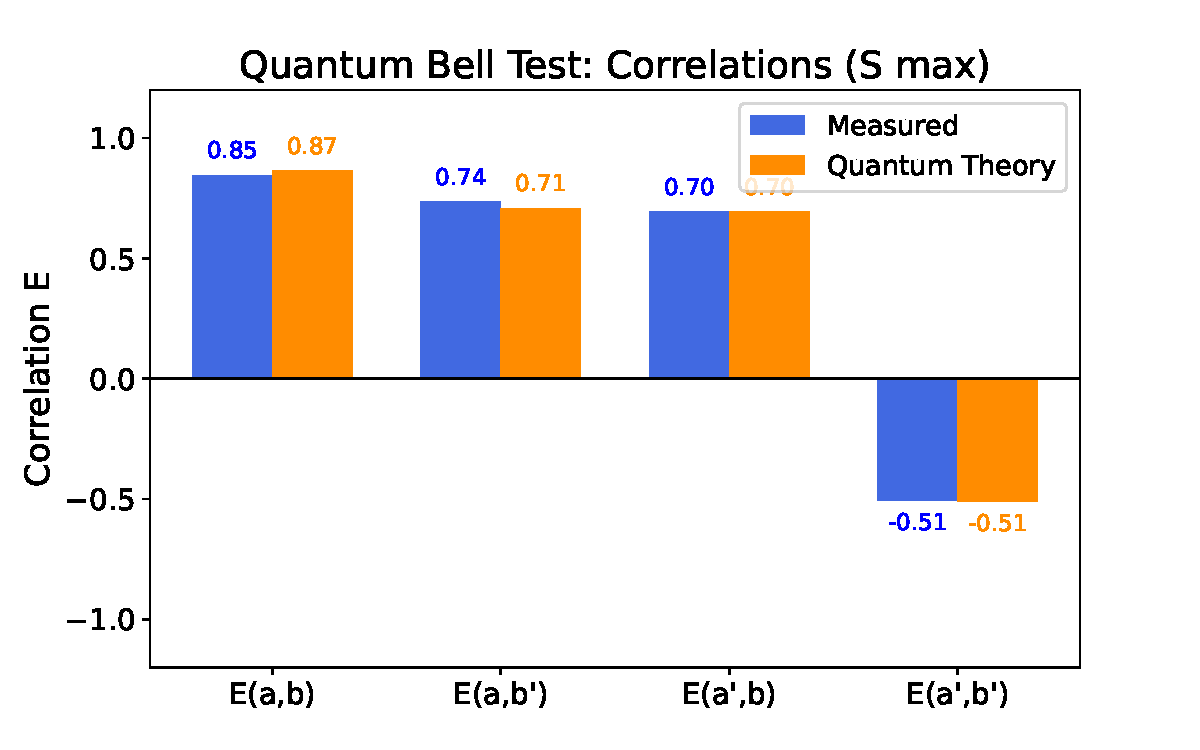
\includegraphics[width=0.75\textwidth]{Figures/correlations_S_max.pdf}
        \caption{Correlaciones medidas vs. teóricas en la iteración óptima ($S_{\max}$).}
    \end{figure}

    \item \textbf{Valor CHSH de $S$ (\texttt{CHSHvalue\_S\_max.pdf}):}  
    Gráfico de una barra única mostrando el valor de $S$ medido en el caso óptimo, con líneas de referencia en $S=2$ (límite clásico) y $S=2\sqrt{2}$ (máximo cuántico).
    
    \begin{figure}[H]
        \centering
        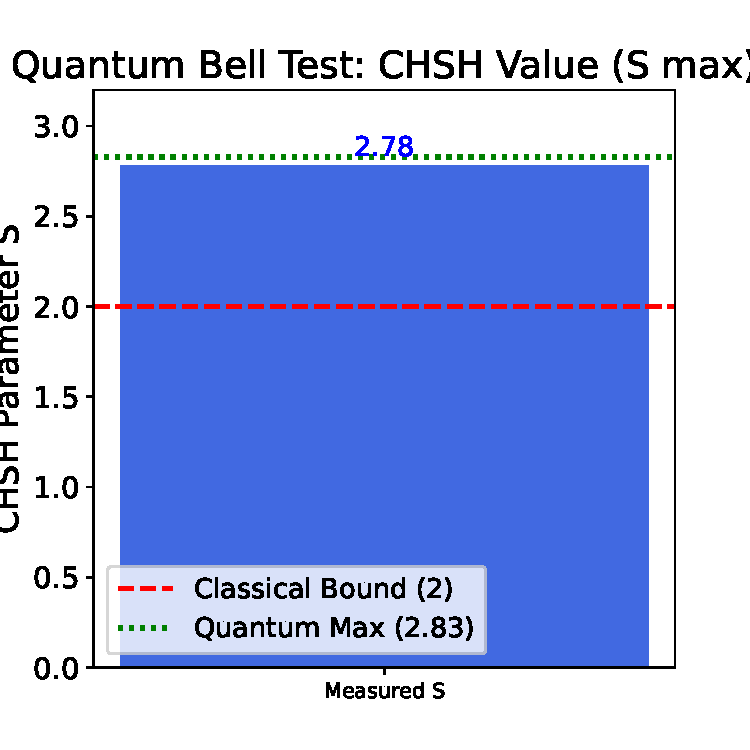
\includegraphics[width=0.55\textwidth]{Figures/CHSHvalue_S_max.pdf}
        \caption{Valor de $S$ en el caso óptimo, con límites clásico y cuántico.}
    \end{figure}

    \item \textbf{Distribución de $S$ (\texttt{Distribution\_S.pdf}):}  
    Histograma con todas las iteraciones (10000 realizaciones), mostrando cuántas veces se alcanzan valores cercanos a los límites clásico y cuántico. Este gráfico ilustra la dispersión estadística de los resultados.
    
    \begin{figure}[H]
        \centering
        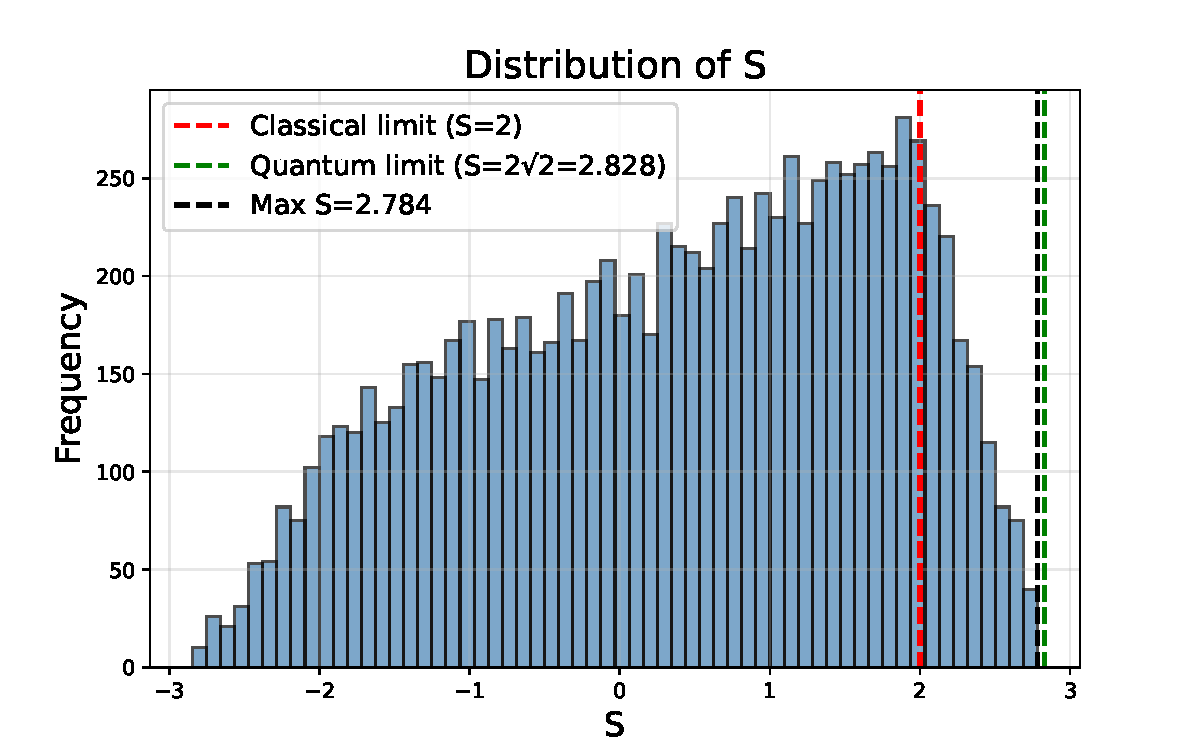
\includegraphics[width=0.75\textwidth]{Figures/Distribution_S.pdf}
        \caption{Distribución estadística de los valores de $S$ a lo largo de todas las simulaciones.}
    \end{figure}

    \item \textbf{Evolución temporal de $S$ (\texttt{AllModels\_S.pdf}):}  
    Diagrama de dispersión que representa los valores de $S$ obtenidos en cada iteración. Se resalta con un asterisco rojo la iteración con $S_{\max}$, esto indica en que numero de iteracion lo alzanzamos, no sera siempre la misma iteracion debido a la naturaleza probabilista que introdujimos.
    
    \begin{figure}[H]
        \centering
        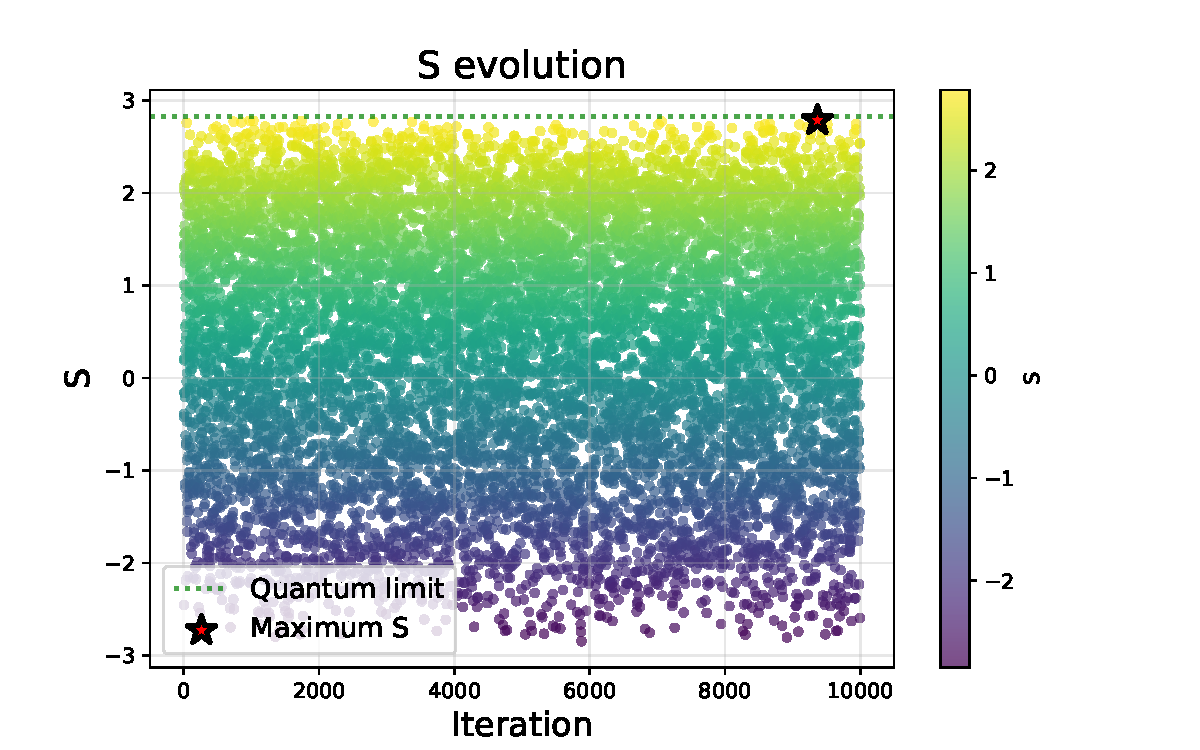
\includegraphics[width=0.75\textwidth]{Figures/AllModels_S.pdf}
        \caption{Evolución de los valores de $S$ en cada iteración de la optimización.}
    \end{figure}

    \item \textbf{Correlaciones en función de $S$ (\texttt{E\_S.pdf}):}  
    Cuatro diagramas de dispersión, uno para cada correlación ($E(a,b)$, $E(a,b')$, $E(a',b)$ y $E(a',b')$), contra los valores de $S$. Esto permite estudiar la dependencia de las correlaciones elementales en la magnitud de la violación.
    
    \begin{figure}[H]
        \centering
        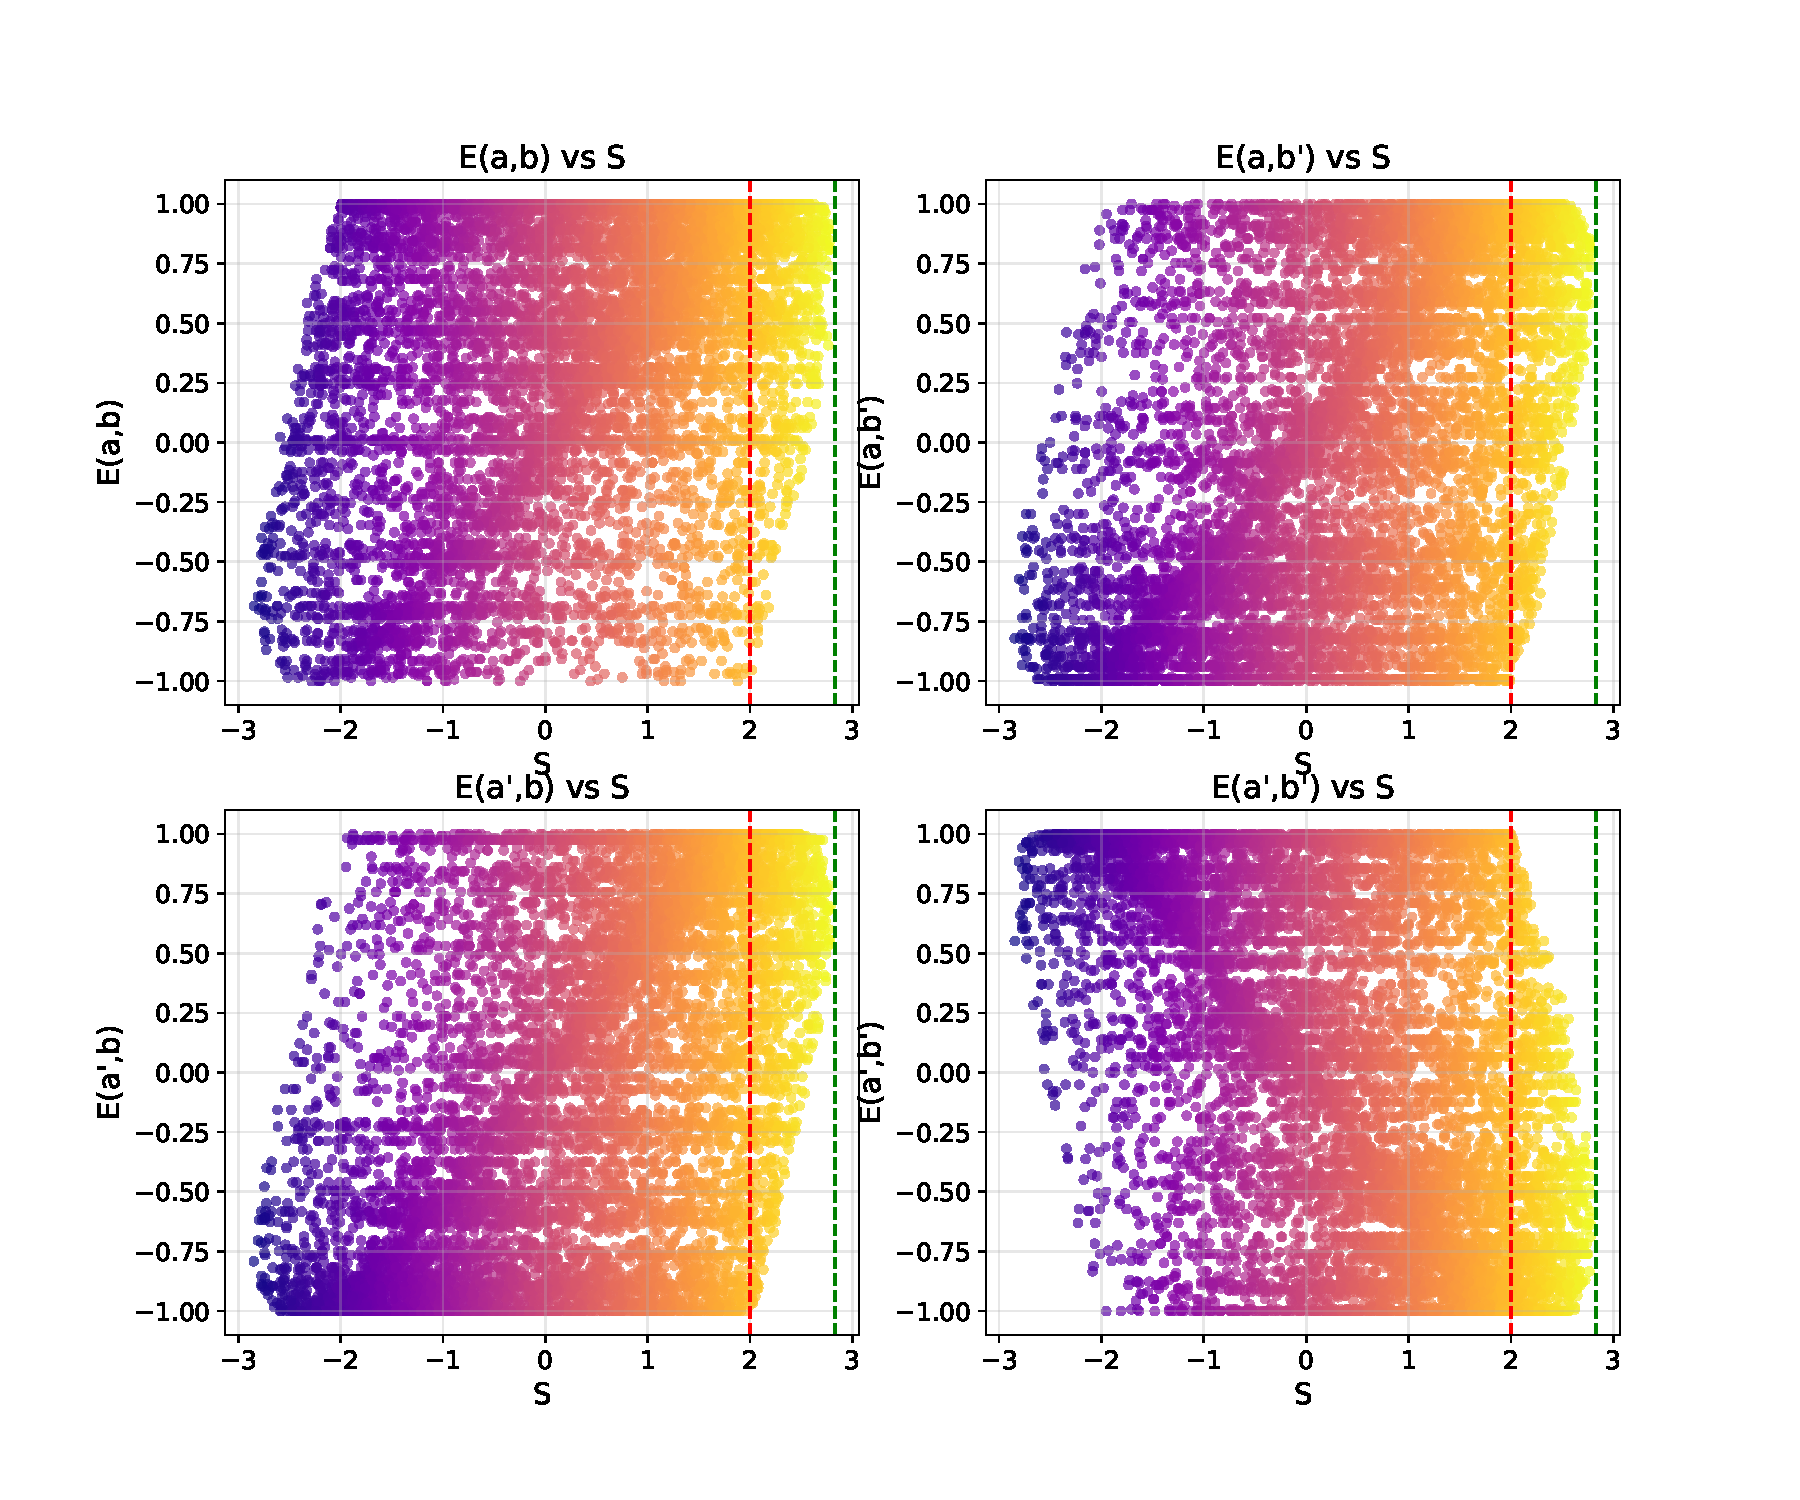
\includegraphics[width=0.95\textwidth]{Figures/E_S.pdf}
        \caption{Relación entre cada correlación elemental $E$ y el valor de $S$ alcanzado.}
    \end{figure}
\end{itemize}


\subsection*{4. Conclusión del análisis}
La función \texttt{analizar\_resultados} complementa el proceso de simulación al proporcionar un conjunto de indicadores gráficos y numéricos que permiten no solo identificar la mejor configuración de ángulos, sino también evaluar la distribución estadística de las violaciones de Bell en un gran número de simulaciones. Los resultados visuales confirman que el programa implementado reproduce la predicción cuántica del estado de Bell $\ket{\Phi^+}$, alcanzando valores de $S$ consistentes con el límite teórico $2\sqrt{2}$.





\section{Notas}

\begin{itemize}
    \item Es importante notar que para todas las bases se mantuvieron las bases tanto para Alice y Bob, asi como, el numero de mediciones (1000).
    \item Todo el código fuente y los scripts pueden ser encontrados en el siguiente \href{https://github.com/LukasWolff2002/TAREA_4_QM}{link}
\end{itemize}

\end{document}